\documentclass[12pt, letterpaper]{article}

\usepackage{graphicx}
\usepackage[margin=1in]{geometry}
\usepackage{bbold}

\graphicspath{{img/}}

\title{Updates for Juanjo}
\date{}

\begin{document}
%\maketitle
\section{Comparison between optimizers}

\begin{figure}[h]
    \centering
    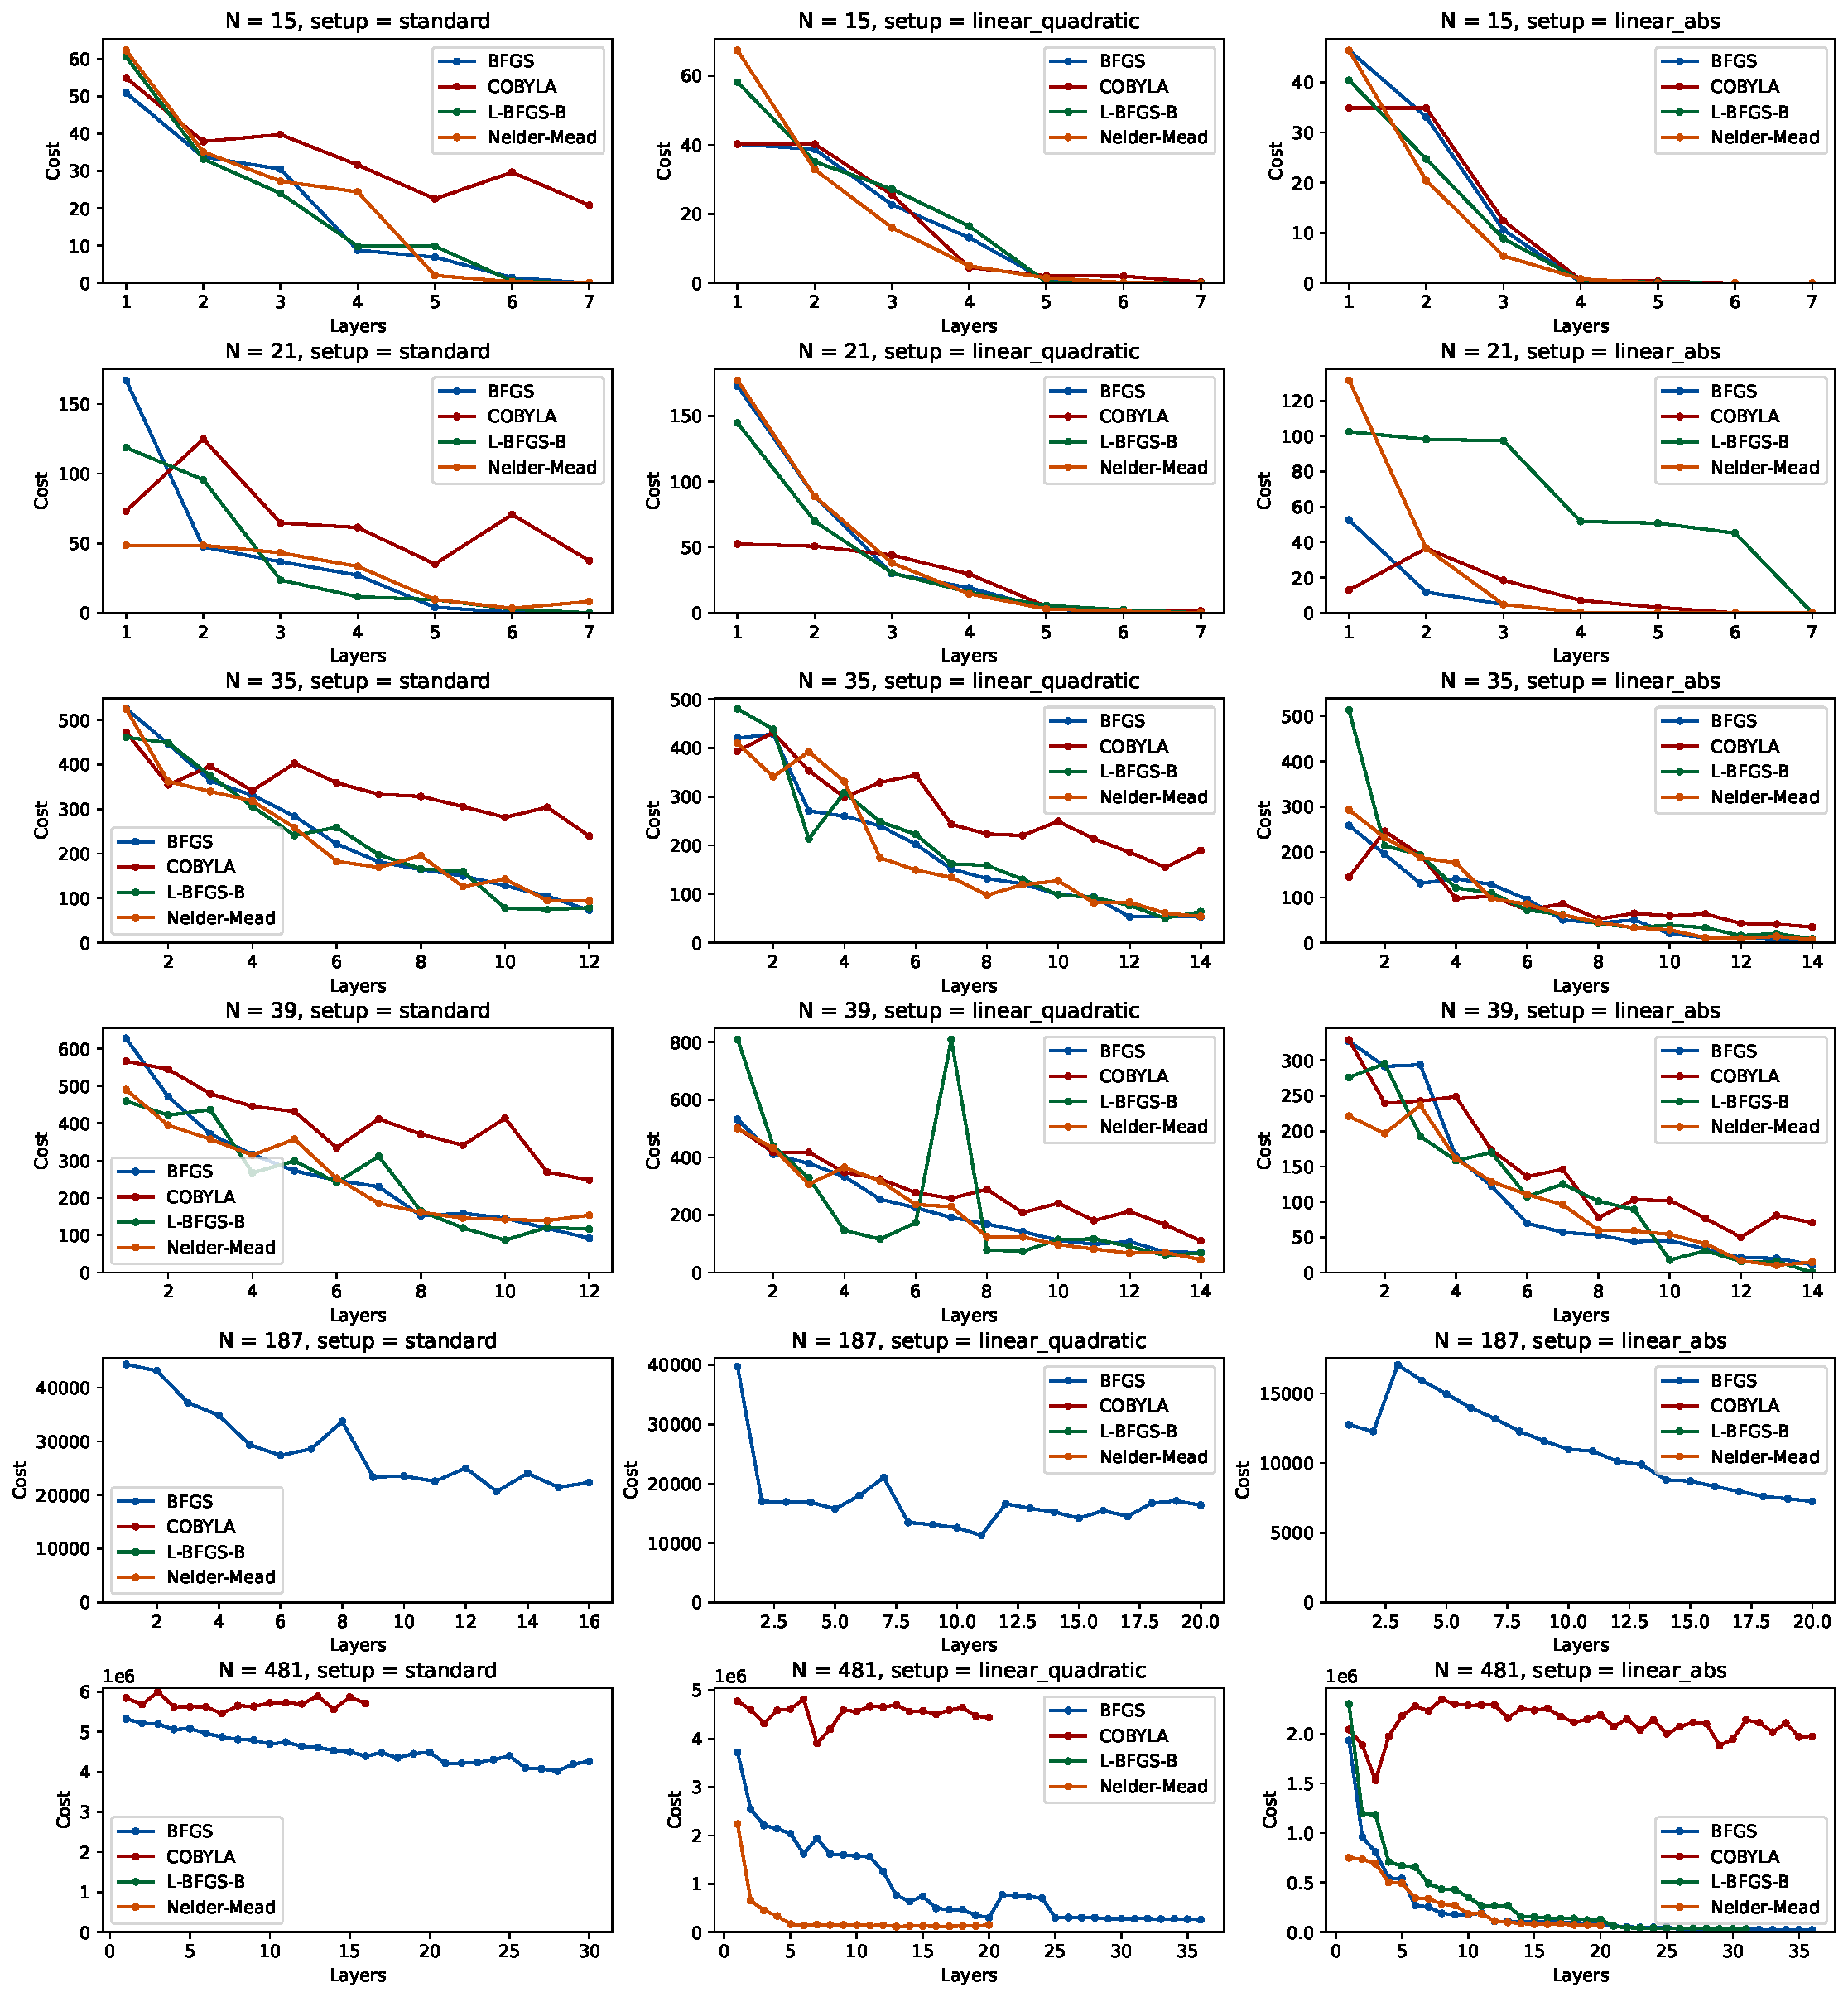
\includegraphics[width=0.9\textwidth]{methods_comparison.pdf}
    \caption{Normalized cost vs layers for different numbers and optimizers}
\end{figure}


\pagebreak
\section{Comparison between setups}
We define the following setups:
\begin{itemize}
    \item \textbf{standard}: quadratic Hamiltonian for evolution and quadratic Hamiltonian for cost evaluation.
    \item \textbf{linear\_quadratic}: linear Hamiltonian for evolution and quadratic Hamiltonian for cost evaluation.
    \item \textbf{linear\_abs}: linear Hamiltonian for evaluation and absolut value Hamiltonian for cost evaluation.
\end{itemize}

\noindent Where
\begin{itemize}
    \item Quadratic Hamiltonian: $\hat{H}_{\mathrm{Q}} = \left[ N\mathbb{I} - \left(\sum_{\ell=1}^{n_p} 2^{\ell} \hat{x}_{\ell} + \mathbb{I} \right)\left(\sum_{m=1}^{n_q} 2^{m} \hat{y}_{m} + \mathbb{I} \right)\right]^2$
    \item Linear Hamiltonian: $\hat{H}_{\mathrm{L}} = \left[ N\mathbb{I} - \left(\sum_{\ell=1}^{n_p} 2^{\ell} \hat{x}_{\ell} + \mathbb{I} \right)\left(\sum_{m=1}^{n_q} 2^{m} \hat{y}_{m} + \mathbb{I} \right)\right]$
\end{itemize}

\begin{figure}[h]
    \centering
    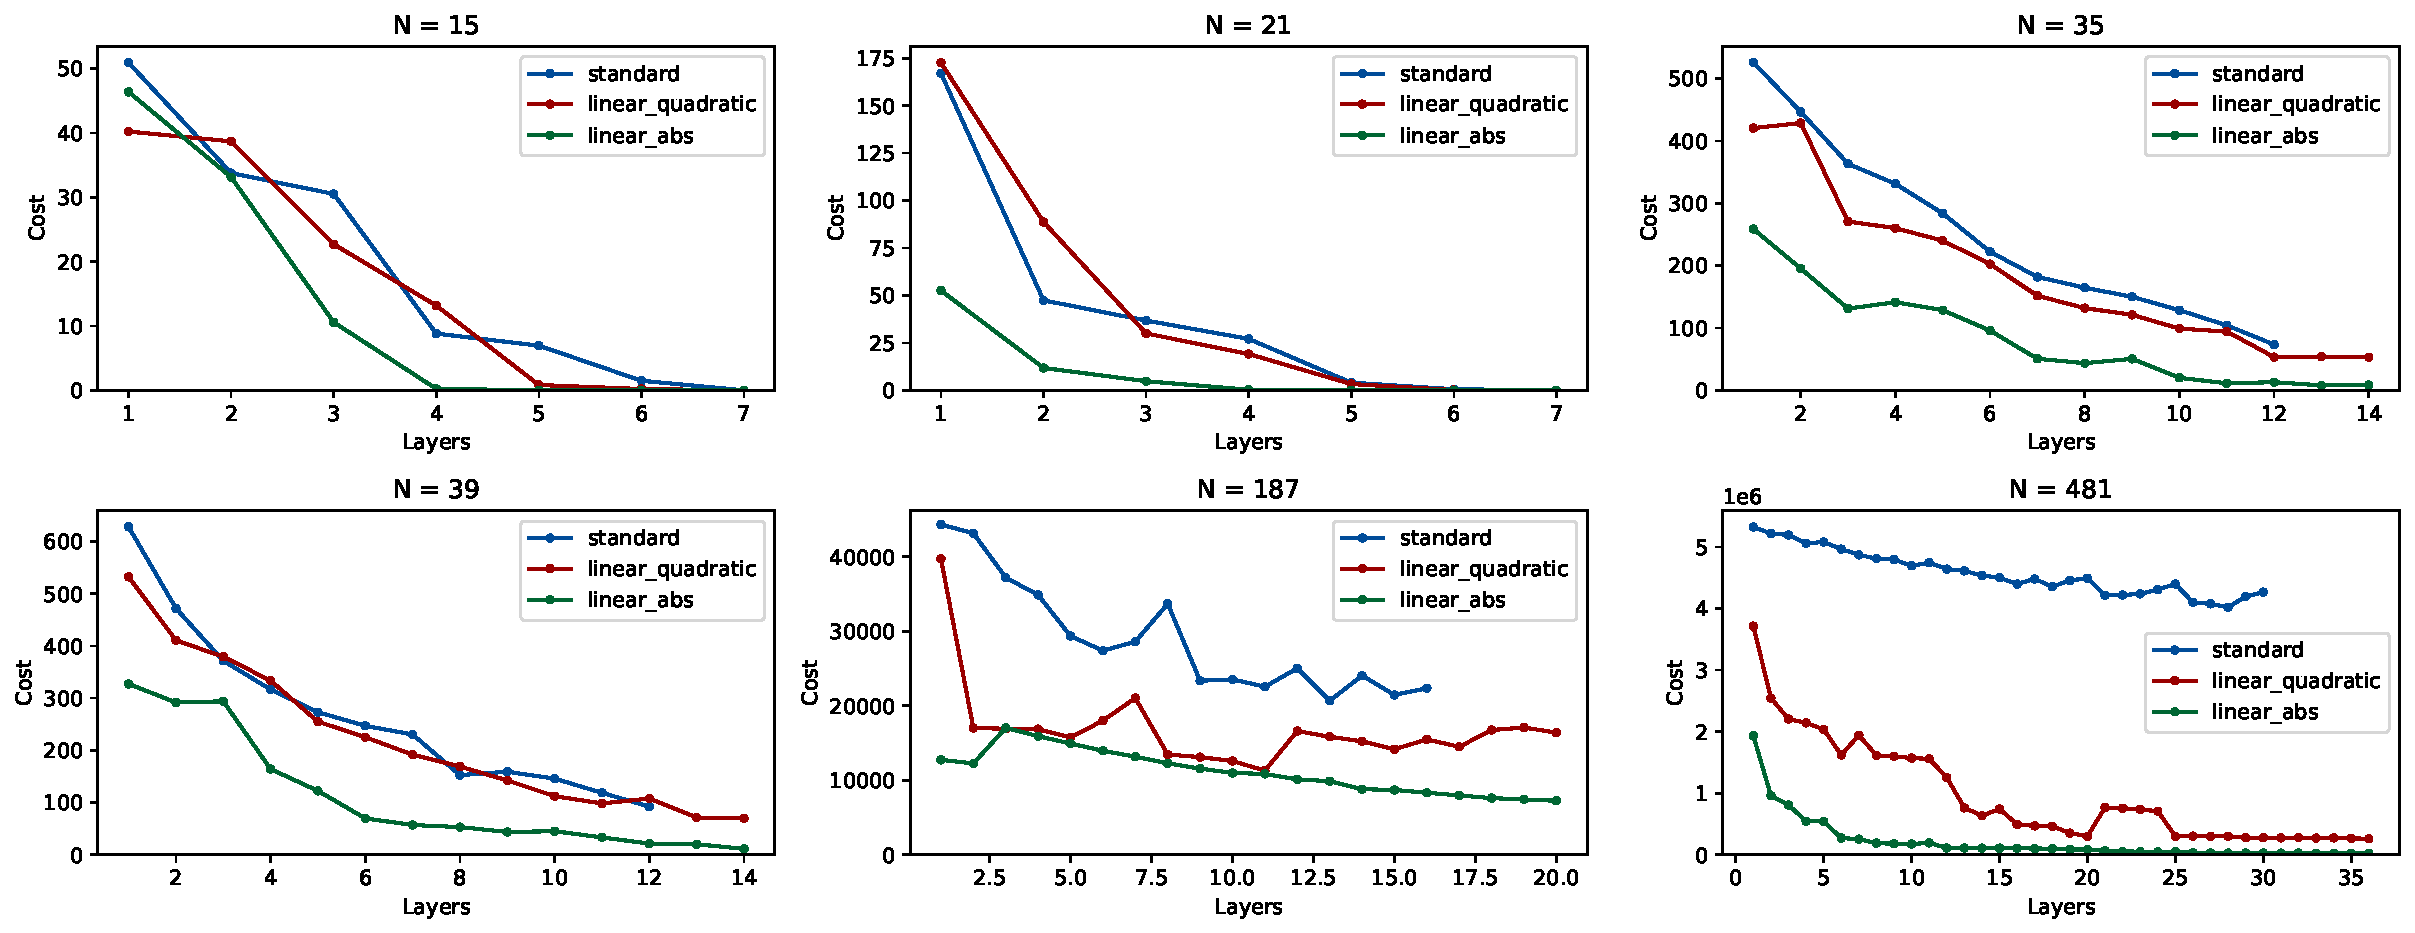
\includegraphics[width=1\textwidth]{setups_comparison.pdf}
    \caption{Normalized cost vs layers for different numbers and setups.}
\end{figure}


\pagebreak
\section{Populations}

\begin{figure}[h]
    \centering
    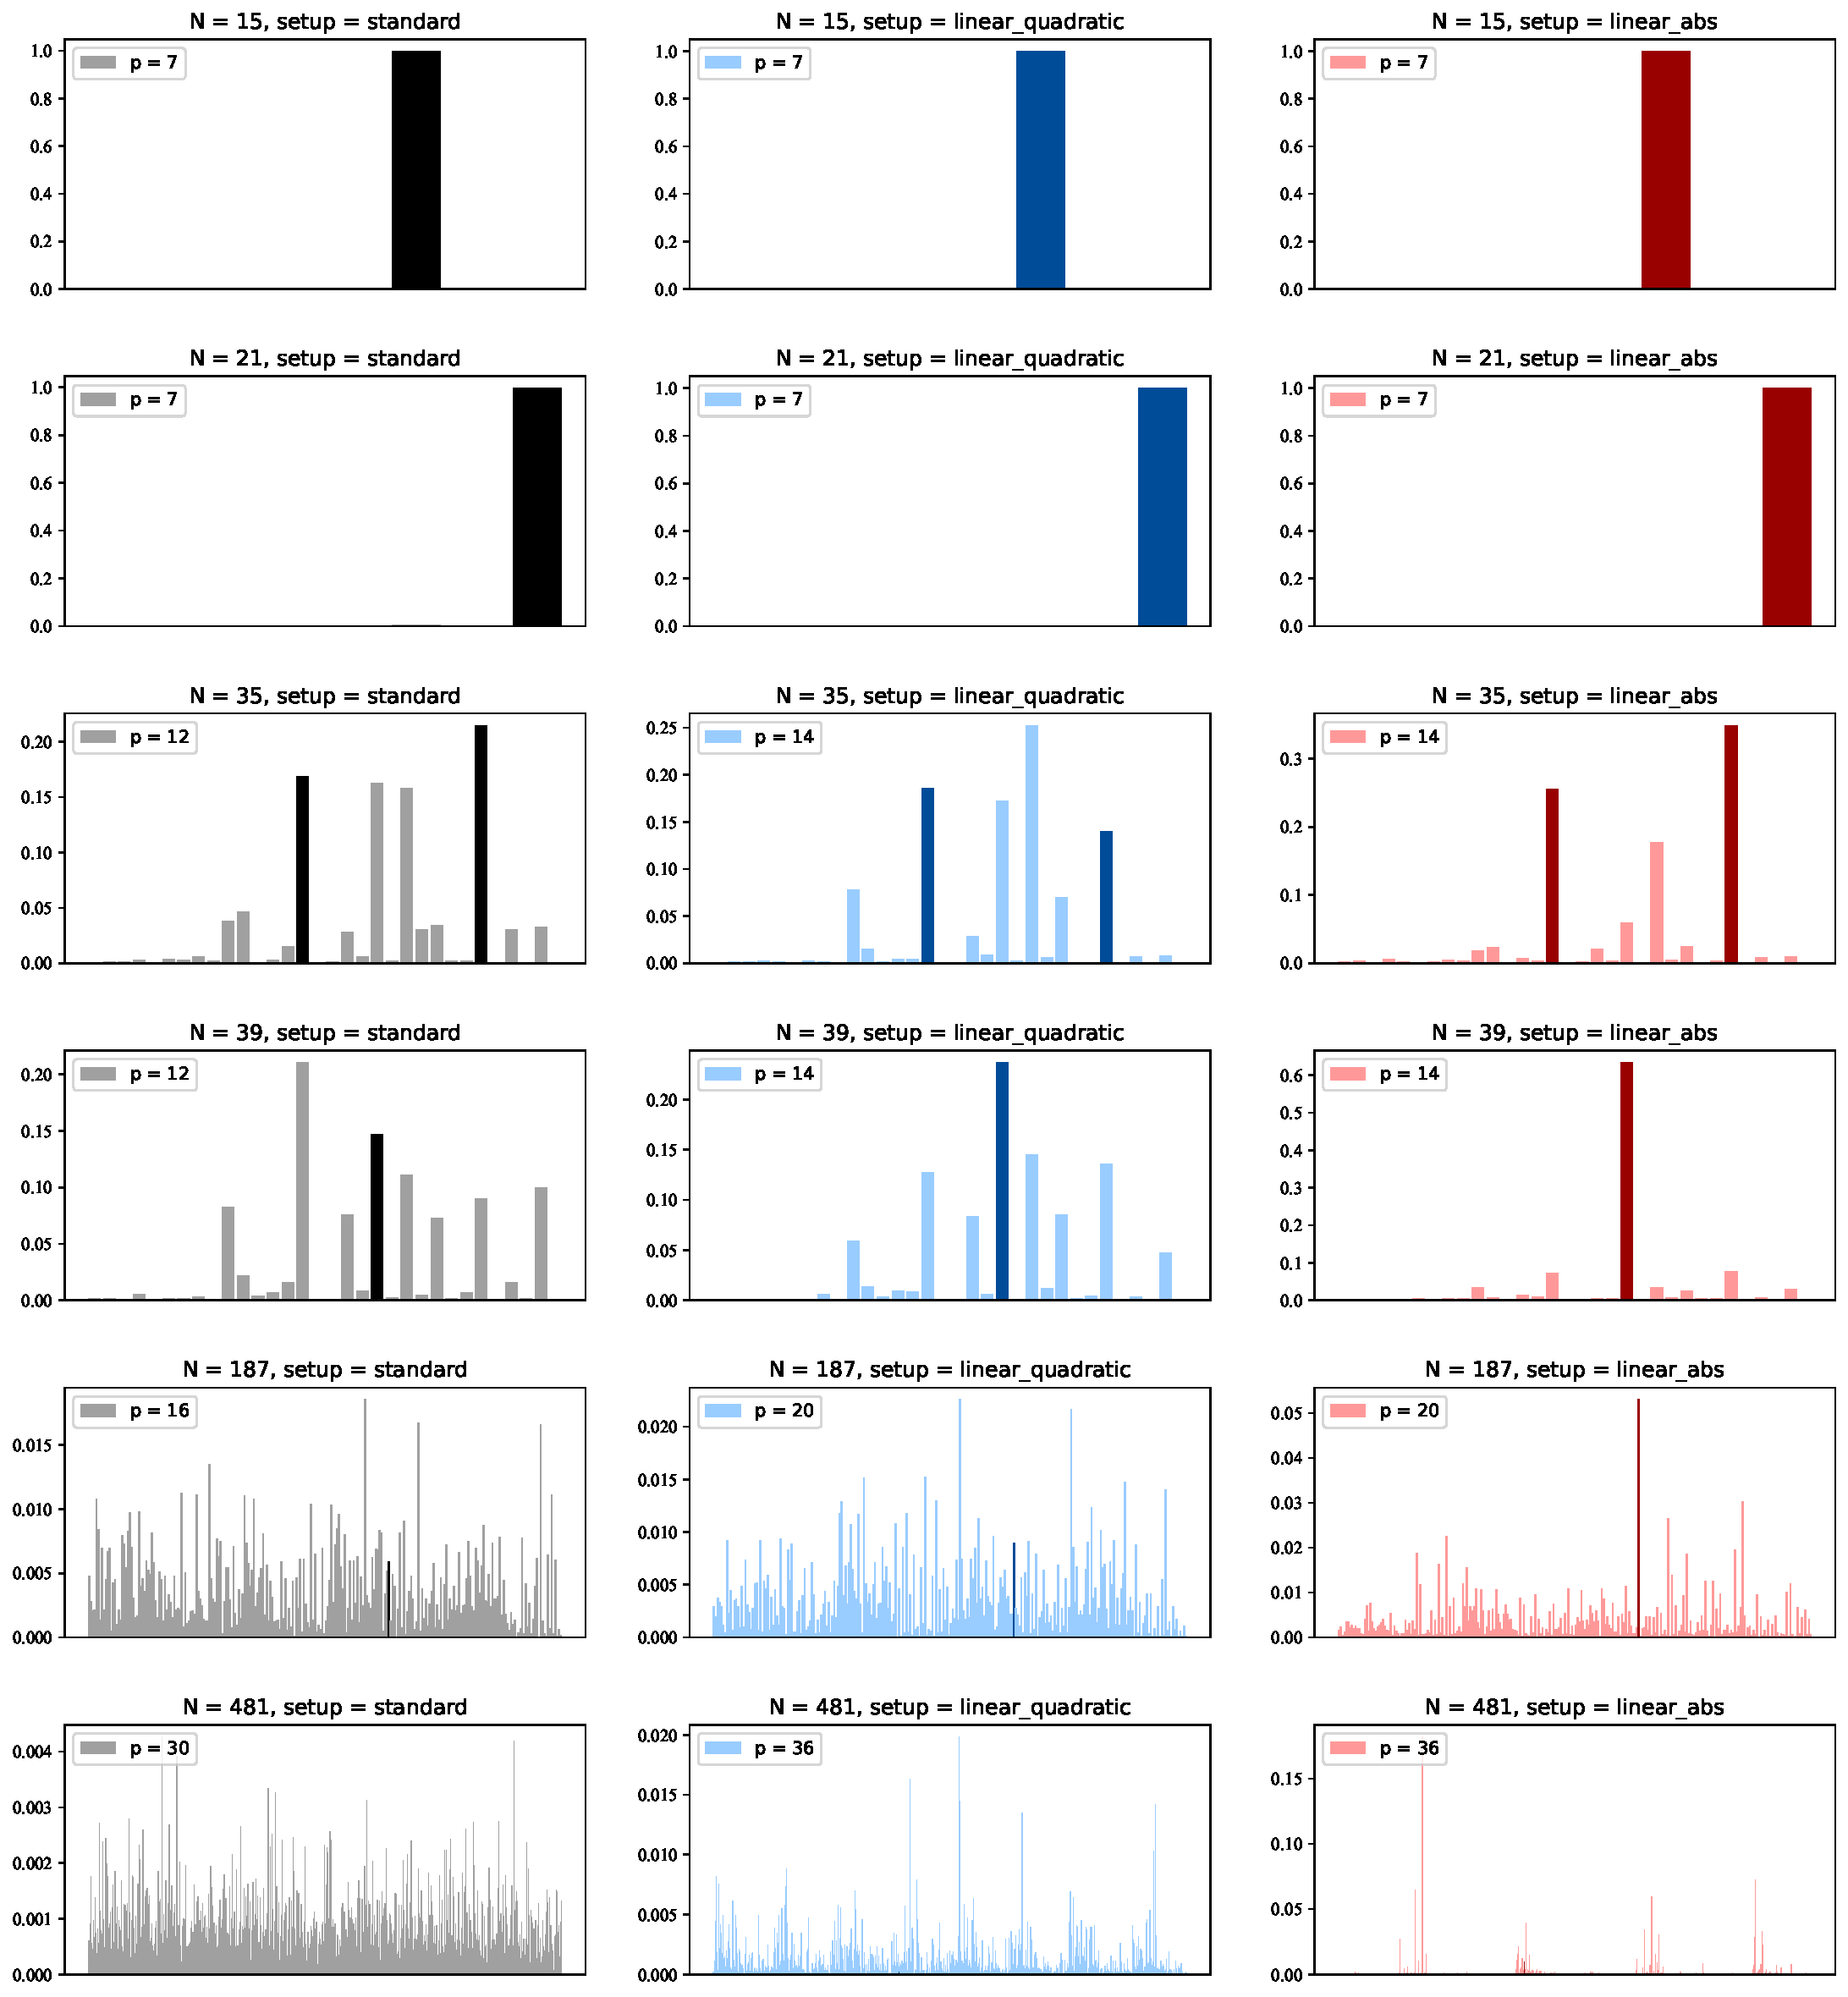
\includegraphics[width=0.9\textwidth]{analysis_populations.pdf}
    \caption{Average populations for different numbers and setups. The dark-colored bars represent the solution. The solutions are clearly identified except for 481.}
\end{figure}

\end{document}